\chapter{Exercise 06}
%******************************************************************************%
%                                                                              %
%                                 Interlude                                    %
%                         for Machine Learning module                          %
%                                                                              %
%******************************************************************************%

\section*{Interlude - Evaluate}

\begin{figure}[h!]
  \centering
  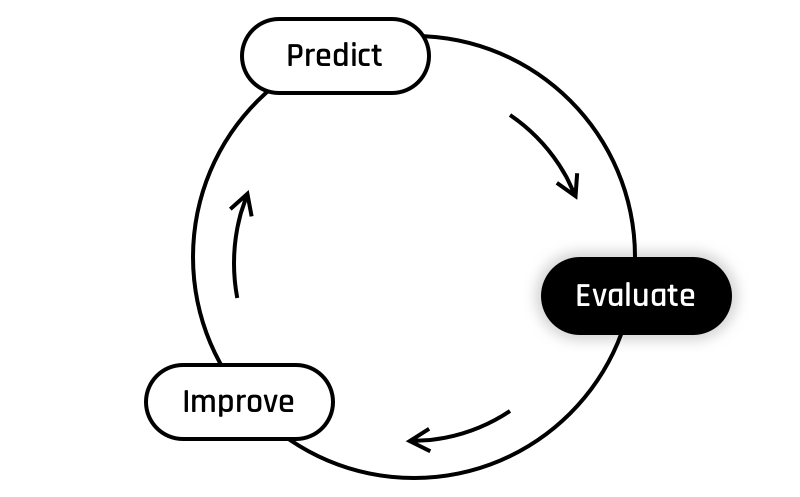
\includegraphics[scale=0.25]{assets/Evaluate.png}
  % \caption{cycle evaluate}
\end{figure}

\subsection*{Introducing the loss function}

How good is our model?  
It is hard to say just by simply looking at the plots!
We can clearly observe that certain regression lines seem to fit the data better than others, but it would be convenient to find a way to measure it. 

\begin{figure}[h!]
  \centering
  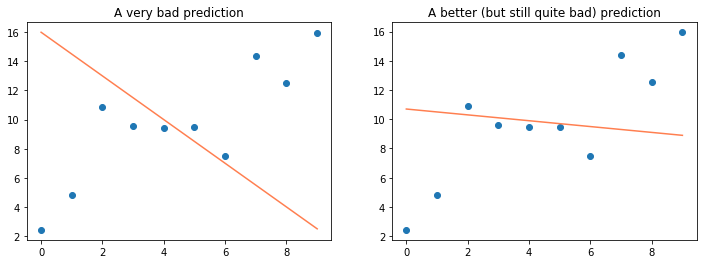
\includegraphics[scale=0.55]{assets/bad_prediction.png}
  \caption{bad prediction}
\end{figure}

To evaluate our model, we are going to use a \textbf{metric} called \textbf{the loss function} (sometimes called \textbf{cost function}).\\
\newline
The loss function tells us how bad our model is performing, how much it \textit{costs} us to use it, how much information we \textit{lose} when we use it.
If the model is good, we won't lose that much; if it's terrible instead, we will have a high loss!

The metric you choose will deeply impact the evaluation (and therefore also the training) of your model.

A frequent way to evaluate the performance of a regression model is to measure the distance between each predicted value ($\hat{y}^{(i)}$) and the real value it tries to predict (${y}^{(i)}$). The distances are then squared, and averaged to get one single metric, denoted $J$:

$$
J(\theta) = \frac{1}{2m}\sum_{i=1}^{m}(\hat{y}^{(i)} - y^{(i)})^2
$$

The smaller, the better! 

\begin{figure}[h!]
  \centering
  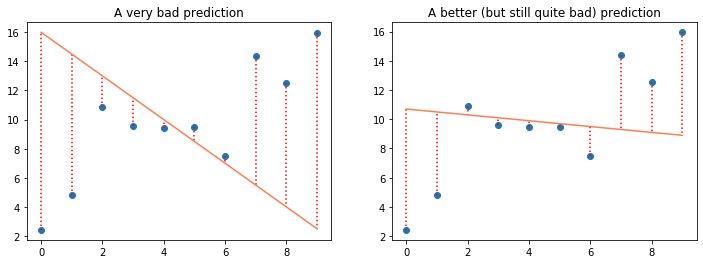
\includegraphics[scale=0.55]{assets/bad_pred_with_distance.png}
  \caption{bad prediction with distance}
\end{figure}

\newpage
\extitle{Loss function}
\turnindir{ex06}
\exnumber{06}
\exfiles{loss.py}
\exforbidden{None}
\makeheaderfilesforbidden


% ================================= %
\section*{Objective}
% --------------------------------- %
Understand and manipulate the notion of loss function in machine learning.

You must implement the following formula as a function (and another one very close to it):

$$
J(\theta) = \frac{1}{2m}\sum_{i=1}^{m}(\hat{y}^{(i)} - y^{(i)})^2
$$

Where:
\begin{itemize}
  \item $\hat{y}$ is a vector of dimension $m\times 1$, the vector of predicted values
  \item $y$ is a vector of dimension $m\times 1$, the vector of expected values
  \item $\hat{y}^{(i)}$ is the ith component of vector $\hat{y}$,
  \item $y^{(i)}$ is the ith component of vector $y$,
\end{itemize}

\newpage

% ================================= %
\section*{Instructions}
% --------------------------------- %
The implementation of the loss function has been split in two functions:
\begin{itemize}
  \item \texttt{loss\_elem\_()}, which computes the squared distances for all examples ($\hat{y}^{(i)} - y^{(i)})^2$),
  \item \texttt{loss\_()}, which averages the squared distances of all examples (the $J_(\theta)$ above).
\end{itemize}

In the loss.py file create the following functions as per the instructions given below:
\par
\begin{minted}[bgcolor=darcula-back,formatcom=\color{lightgrey},fontsize=\scriptsize]{python}
def loss_elem_(y, y_hat):
	"""
	Description:
		Calculates all the elements (y_pred - y)^2 of the loss function.
	Args:
      y: has to be an numpy.array, a two-dimensional array of shape m * 1.
      y_hat: has to be an numpy.array, a two-dimensional array of shape m * 1.
	Returns:
		J_elem: numpy.array, a array of dimension (number of the training examples, 1).
		None if there is a dimension matching problem.
		None if any argument is not of the expected type.
	Raises:
		This function should not raise any Exception.
	"""
	... your code here ...

def loss_(y, y_hat):
	"""
	Description:
		Calculates the value of loss function.
	Args:
      y: has to be an numpy.array, a two-dimensional array of shape m * 1.
      y_hat: has to be an numpy.array, a two-dimensional array of shape m * 1.
	Returns:
		J_value : has to be a float.
		None if there is a dimension matching problem.
		None if any argument is not of the expected type.
	Raises:
		This function should not raise any Exception.
	"""
	... your code here ...
\end{minted}

% ================================= %
\section*{Examples}
% --------------------------------- %
\begin{minted}[bgcolor=darcula-back,formatcom=\color{lightgrey},fontsize=\scriptsize]{python}
import numpy as np

x1 = np.array([[0.], [1.], [2.], [3.], [4.]])
theta1 = np.array([[2.], [4.]])
y_hat1 = predict_(x1, theta1)
y1 = np.array([[2.], [7.], [12.], [17.], [22.]])

# Example 1:
loss_elem_(y1, y_hat1)

# Output:
array([[0.], [1], [4], [9], [16]])

# Example 2:
loss_(y1, y_hat1)

# Output:
3.0

x2 = np.array([0, 15, -9, 7, 12, 3, -21]).reshape(-1, 1)
theta2 = np.array(np.array([[0.], [1.]]))
y_hat2 = predict_(x2, theta2)
y2 = np.array([2, 14, -13, 5, 12, 4, -19]).reshape(-1, 1)

# Example 3:
loss_(y2, y_hat2)

# Output:
2.142857142857143

# Example 4:
loss_(y2, y2)

# Output:
0.0
\end{minted}

\info{
  This loss function is very close to the one called \textbf{"Mean Squared Error"}, which is frequently mentioned in Machine Learning resources.
  The difference is in the denominator as you can see in the formula of the $MSE = \frac{1}{m}\sum_{i=1}^{m}(\hat{y}^{(i)} - y^{(i)})^2$.
  
  Except the division by $2m$ instead of $m$, these functions are rigourously identical: $J(\theta) = \frac{MSE}{2}$.  
  
  MSE is called like that because it represents the mean of the errors (i.e.: the differences between the predicted values and the true values), squared.
  
  You might wonder why we choose to divide by two instead of simply using the MSE?  
  \textbf{(It's a good question, by the way.)}
  \begin{itemize}
    \item First, it does not change the overall model evaluation: if all performance measures are divided by two, we can still compare different models and their performance ranking will remain the same.
    \item Second, it will be convenient when we will calculate the gradient tomorow. Be patient, and trust us ;)
  \end{itemize}
  }
  